\documentclass[
a4paper,
12pt,
oneside,
headsepline,		% Linie für Kopfzeile
footsepline,		% Linie für Fußzeile
%bibtotoc
]{scrbook}
 
% Druckbereich: \areaset[BCOR]{textwidth}{textheight}
% BCOR ist "Binding Correction", also wieviel Innenrand verloren geht
% A4 hat 297mm x 210mm
% wenn keine Marginalien, dann ist Breite 15cm vielleicht besser
% \areaset[1.5cm]{14cm}{25cm}
 \usepackage[left=3cm,right=2cm,bottom=2.5cm]{geometry}
%% Die folgende Zeile sorgt dafür, daß die Fußnoten eingerückt werden,
%% und zwar um 2em (class scrbook).
\deffootnote{2em}{2em}{\textsuperscript{\normalfont\thefootnotemark} }
 
\usepackage[utf8x]{inputenc}  % Unterstützung für Unicode-Zeichen-Eingabe
\usepackage[T1]{fontenc}      % Unterstützung für Europäische-Zeichen-Ausgabe
\usepackage{ae}               % verbesserte Unterstützung für Umlaute
\usepackage[german]{babel}    % deutsche Übersetzungen und Wortumbrüche
\usepackage[scaled]{helvet}  % schönere Schriftart: Helvetica
\usepackage{mathptmx}            % passende Mathe-Schriftart
\usepackage{courier}             % passende Monospaced-Schriftart
\usepackage{pgf}              % Unterstützung für Graphiken
\usepackage{tikz}             % Unterstützung für Graphiken
\usepackage[onehalfspacing]{setspace}
\usepackage{acronym} 
\usepackage{listings}
\usepackage{color}
\usepackage{float}

\definecolor{Gray}{gray}{0.9}
\definecolor{sun1}{rgb}{0.2,0.2,0.4}
\definecolor{sun2}{rgb}{0.4,0.4,0.6}
\definecolor{sun3}{rgb}{0.6,0.6,0.8}
\definecolor{sun4}{rgb}{0.8,0.8,1}
\definecolor{msblau}{rgb}{0.31,0.4,0.517}
\definecolor{darkred}{rgb}{0.5,0,0}
\definecolor{darkgreen}{rgb}{0,0.5,0}
\definecolor{darkblue}{rgb}{0,0,0.5}
 
\usepackage[                
   pdftex,                  % Ausgabe-Medium: PDF
   colorlinks=true,         % farbige Links in der Bildschirm-Version?
   pdfstartview=FitV,       % wie soll Acrobat starten?
   linkcolor=blue,         % Farbe für Querverweise
   citecolor=blue,         % Farbe für Zitierungen
   urlcolor=blue,          % Farbe für Links
   bookmarks=true
   ]{hyperref}              % Paket für Links im PDF
 
%%%% Informationen über den Text festlegen %%%%%%%%%%%%%%%%%%%%%%%%%%%%%%%%%%
\title{Bachelorarbeit}
\author{Andreas Collmann}
\date{\today}
 
%%% hier können noch viel viel mehr Einstellungen kommen
%%%% hier beginnt der Inhalt %%%%%%%%%%%%%%%%%%%%%%%%%%%%%%%%%%%%%%%%%%%%%%%%
%\spacing{1.5}

\makeindex

\newcommand{\eruck}[1]{
    \noindent\hspace*{#1}
}
\newcommand{\zab}[1]{
    \vspace*{#1}
}
\newcommand{\fina}[1]{
    {\em #1}
}
\newcommand{\finar}[1]{
    {\fina{#1}\textsuperscript{\textregistered}}		
}
\newcommand{\sona}[1]{
    {\em #1}
}
\newcommand{\code}[1]{
    {\\ \eruck{20mm} \texttt{#1} \\}
}

% Formatierung Quellcode

\lstset{
    language=Python,
	numbers=left,
	backgroundcolor=\color{Gray},
	basicstyle=\small,
	showspaces=false,
    basicstyle=\scriptsize\ttfamily,
    keywordstyle=\bfseries\ttfamily\color{orange},
    stringstyle=\color{blue}\ttfamily,
    commentstyle=\color{gray}\ttfamily,
    emph={square}, 
    emphstyle=\color{blue}\texttt,
    emph={[2]root,base},
    emphstyle={[2]\color{orange}\texttt},
    showstringspaces=false,
    flexiblecolumns=false,
    tabsize=2,
    numbers=left,
    numberstyle=\tiny,
    numberblanklines=false,
    stepnumber=1,
    numbersep=10pt,
    xleftmargin=15pt
	}

\begin{document}

 %\section*{}
%\newpage
%\addtocounter{page}{-1}
 
 %%%%%%%%%%%%%%%%%%%%%%%%%%% Titelseite %%%%%%%%%%%%%%%%%%%%%%%%%%%%%%%%%%%%%
\begin{titlepage}
  \centering
  \begin{figure}[h]
  \centering
  
\includegraphics[width=0.45\textwidth]{pic/h_da.png}
  %\caption{innoQ \\ Robert-Bosch-Straße 7 \\ 64293 Darmstadt}
  \label{fig:innoq}
  \end{figure}	
  \zab {2cm}
  \textbf{\Large Hochschule Darmstadt} \\	
  \zab {0,4cm}
  {\Large - Fachbereich Informatik -} \\
  \zab {3cm}
  {\large Untersuchung der Offenen Schnittstellen des UR5 Roboters anhand eines Anwendungsbeispiels} \\
  \zab {2cm}
  Abschlussarbeit zur Erlangung des akademischen Grades Bachelor of Science
  (B.Sc.) \\	
  \zab {1cm}
  vorgelegt von \\
  \zab {1cm}
  {\Large Andreas Collmann} \\
  \zab {2cm}
  \begin{tabular}{ll}
  Referent: & Prof. Dr. Horsch\\
  Koreferent: & Prof. Dr. Akelbein\\
  \end{tabular}
\end{titlepage}
 
 \section*{Erklärung}
\label{erklaerung}
		 
Ich versichere hiermit, dass ich die vorliegende Arbeit selbständig verfasst und
keine anderen als die im Literaturverzeichnis angegebenen Quellen benutzt habe.
\zab {0,4cm}\\
Alle Stellen, die wörtlich oder sinngemäß aus veröffentlichten oder noch nicht
veröffentlichten Quellen entnommen sind, sind als solche kenntlich gemacht. \zab
{0,4cm}\\
Die Zeichnungen oder Abbildungen in dieser Arbeit sind
von mir selbst erstellt worden oder mit einem entsprechenden Quellennachweis
versehen. \zab {0,4cm}\\
Diese Arbeit ist in gleicher oder ähnlicher Form noch bei keiner anderen
Prüfungsbehörde eingereicht worden. \zab {2cm}\\
Darmstadt, den 28.03.2014 \\

 \section*{Abstract}
\label{abstract}

Um die Vorteile des kollaborativen Arbeitens von Menschen und Robotern anzuwenden, wird im Zuge dieser Arbeit der für die Kollaboration zugelassene Roboter UR5 der Firma ``Universal Robots'' untersucht. Es wird untersucht, welche Möglichkeiten diesen Roboter zu programmieren möglich sind. Die Untersuchung erfolgt aufgrund einiger Kriterien, die auf den Einsatz mit Kollaboration zielen.
Die Schnittstellen des UR5 Roboters werden untersucht und dokumentiert.
Am Ende dieser Arbeit wird eine Entscheidungsfindung zusammengefasst, welche Schnittstelle zu welchem Anwendungsfall am besten zu wählen ist. Um dies zu evaluieren, wurde eine Beispielanwendung in jeder Schnittstelle entwickelt. Die Ergebnisse sind am Ende knapp zusammengefasst.
 
 \tableofcontents
 \listoffigures
 \listoftables
 \lstlistoflistings
 
 \chapter{Einleitung}
\label{einleitung}

\section{Fachliche Umgebung}
\label{fachliche_domaene}

Hauptaugenmerk dieser Arbeit ist es die möglichkeiten der Roboter-Mensch-Kollaboration
in der Industire, Medizin, Schule mit diesem Roboter zu prüfen.
Inwiefern der Mensch mit einem Heutigen Roboter mit entsprechenden Richtlinen programmiert werden kann um in den entsprechenden Feldern mit dem Menschen zusammen zu Arbeiten.

\section{Motivation und Ziel des Projektes}
\label{projektziel_motivation}

In der Industrie werden Roboter in den Fertigungsanlagen eingesetzt. 
Dies geschiet meist in Koordination mit anderen Robotern. In der nähe dieser Roboter, darf sich kein Mensch aufhalten, die Roboter sind umhaust, sprich in einem speziellen Bereich abgesichert, damit keine unfälle passieren können. 
Auf diese Weise kann man sehr effizient über automatisierte Fließbandstraßen Produkte herstellen.

Wenn jedoch eine sehr filigranere Arbeit gefragt ist, muss das Werkstück von einem Menschen bearbeitet werden, da der Mensch wesentlich bessere Fähigkeiten hat, auf Probleme zu reagieren oder Korrekturen vorzunehmen. In diesem fall wird die Fließbandstraße unterbrochen. Das Produkt muss aus dem umhausten Bereich gebracht werden, wo es von einem Menschen bearbeitet werden kann.

Für die Prodution wäre es viel sinnvoller und zeitsparender, wenn Roboter für den Menschen so sicher sind, dass keine Trennung zwichen Mensch und Robotern existiert.

In dem Bereich Pflege und der Medizin, müssen oft hebe arbeiten ausgeführt werden. Dies fürt dazu, dass die Menschen in solchen Berufen im späteren Altag mit Rückenproblemen oder ähnliche leiden leben müssen. Roboter, die eingesetzt werden um diese lasten abzunehmen, würde die Arbeit erleichtern und verletzungen vorbeugen.

Es soll untersucht werden inwiefern die Zusammenarbeit von Robotern und Menschen mit einem Roboter der die Sicherheitsauflagen erfüllt, realisiert werden kann.

\section{Aufgabenstellung}
\label{aufgabenstellung}

Es soll ein Anwendungsprogramm für alle möglichen Programmierschnittstellen für den Ur5 Roboter von Universal Robots entwickelt werden.
Dieses Anwendungsprogramm soll so ausgelegt sein, dass es als eine Beispielanwendung einer Roboter-Mensch Kollaboration ist.
Diese verschiedenen Programme werden miteinander verglichen. Es soll eine Entscheidungshilfe gegeben werden, für welchen Anwendungsfall, welche Schnittstelle am besten geeignet ist.

Die Programmierschnittellen sollen möglichst gut dokumentiert werden.

\section{Einordnung in die Themenfelder der Informatik}
\label{sec:einordnung}

Die Schnittstellen werden mit den Standart Programmiersprachen C/C++ und Python programmiert. Hinzu kommt noch von die eigens von Universal Robots entwickelte URScript sprache.
Da versucht wird den Roboter von einem anderen Rechner zu steuern, wird auch Netzwerkprogrammierung benötigt. Es muss eine kleines Protokoll entwickelt werden, mit dem der Roboter kommunizieren kann um Anwenderdaten zu speichern. 

 \chapter{Grundlagen}

\section{Roboter-Mensch-Kollaboration}
\label{sec:roboter-mensch-kollaboration_gru}

Man unterscheidet die Arbeiten mit einem Roboter unter mehrere Arten.
Roboter die mit anderen Robotern gleichzeitig arbeiten nennt man Kooperation zwichen Robotern.
Der Mensch ist in diesem Arbeitsumfeld nicht dabei und kann nur von außen einfluss nehmen.
\\\\
Als nächstes gibt es die Kollaboration zwichen dem Roboter und dem Mensch. 
Hier wird auch eine Unterteilung vorgenommen die unterschiedliche Richtlinien erfordern.

\begin{itemize}
\item Sicherhaltshalt, wenn der Mensch den Kollaborationsraum betritt.
\item Dauerhafte Überwachung des abstands zwichen Mensch und Roboter, der mit reduzierter geschwindigkeit arbeitet.
\item Verminderte Geschwindigeit. Führung des Roboters durch den Mensch. Sensoren erfassen die kräfte, die vom Menschen ausgeführt werden und übertragen sie auf den Roboter.
\item Beschränkung der im Roboter ausgeführten Energie. Überwachung des Roboters auf Kollision und sofortigem Stop
\end{itemize}

\subsection{Richtlinien}
\label{kol_richtlinien_gru}

In so gut wie allen fällen sind Roboter in der Industrie in einem extra abgesicherten Bereich umzäunt, damit kein Arbeiter sich verletzen kann. Diese Robote sind umhaust. Es ist nicht möglich in einem gemeinsamen Arbeitsbereich zu kollaborieren. 
Damit Menschen im Arbeitsbereich vom Robotern Arbeiten dürfen müssen diese Roboter bestimmte Sicherheitsrichtlinien entsprechen.
Der Roboter darf unter keinen Umständen eine Lebensbedrohliche gefahr darstellen. Die Norm ISO 10218

\section{Ur5 Roboter}
\label{sec:ur_robot_gru}

Die Dänische Firma Universal Robots hat den leichten Ur5 und mittelgroßen Ur10 Roboter hergestellt mit erfüllbaren Normen um mit diesem Roboter zu kollaborieren. Man kann sich im laufenden Betrieb in der Nähe aufhalten um Wegpunkte zu Teachen oder auch gleichzeitig an einem Werkstück zu arbeiten. 

\subsection{Eigenschaften}
\label{ur_eigenschaften_gru}

Der Roboter besitzt 6 Gelenke die ihm ermöglichen einen 360° Arbeitsbereich mit einem Radius von ca 85cm zu ermöglichen. Gesteuert wird er von einem Linux Rechner, der sich in der Nähe befindet. 
Die Festplatte für das System ist eine Speicherkarte, die leicht ausgetauscht werden kann.
\\\\
Um den Rechner anzusprechen existiert bei lieferung ein Touch Tablet, das für das Linux System den Visuellen Output gibt. bei Start wird auch automatisch die Software für den Roboter gestartet. Die Software nennt sich Polyscope und wurde in Java geschrieben. Diese Software verbindet sich per TCP/IP auf den URController. Ein Server Programm das die Schnittstelle von dem Linux System zu dem Roboter Controller auf dem Rechner Herstellt.
\\\\
Die Polyscope Software läuft im normalen Modus und den Administrativen Modus. Der Normale Modus ermöglicht es Programme zu erstellen, laufen zu lassen und Grundeinstellungen vorzunehmen. Außerdem kann ein Software Update der Polyscope Software gemacht werden.

\subsection{System Aktualisieren}
\label{ur_update_gru}

Zwei Arten von Updates sind hier zu unterscheiden. Zum einen kann das Linux System geupdatet werden. Auf normalem wege über den Packetmanager des Systems, oder wenn man das neuste Image von Universal Robots runterläd und dann das System neu aufspielt. Hier ist jedoch zu beachten, dass dabei alle Daten verloren gegangen werden. Deshalb sollte eine Datensicherung vorgenommen werden. Wie dies geschieht wird im darauf folgenden Unterkapitel beschrieben(\ref{ur_datensicherung_gru}).
\\\\
Updates für dem Roboter müssen allerdings manuell gemacht werden. Hierfür müssen die aktuellen Updates von der Homepage von Universal Robots runtergeladen werden. Die Update-Datei muss mit der dateiendung .urup auf einen USB Stick mit einem FAT32 Dateisystem abgelegt werden.\\\\
Nachdem der USB Stick an das Linuy System angeschlossen ist, kann von der Polyscope Software das Update ausgeführt werden. Einstellungen->Updates.\\
Im Administrativen Modus können nach dem Update die Firmware's der einzelnen Gelenkcontroller geupdatet werden. Die werden im Update mitgeliefert. Die einzelnen Schritte sind in den Dokumentationen beiliegend auf der CD zu finden.

\subsection{Datensicherung}
\label{ur_datensicherung_gru}

Die Daten des Roboters sind abgelegt in root verzeichniss unter 

\begin{lstlisting}[caption={Pfade Der Ur5 Relevanten Dateien}, label=lst:ur5data ,captionpos=b] 
/root/.urcontrol    #Konfigurationsdateien des Ur5Roboters
/programs   		#alle geschriebenen Programme unter Polyscope
\end{lstlisting}

Es ist möglich die Dateien per USB Stick zu sichern oder über Programme wie ``SCP'' über das Netzwerk zu Kopieren.

\section{Übersicht der Programmierschnittstellen}
\label{sec:programm_api_uebersicht_gru}

Der Ur5 Roboter kann auf drei Ebenen angesprochen werden.\\

\begin{itemize}
\item Polyscope
\item URscript
\item C-Api
\end{itemize}

\begin{figure}[ht]
  \centering
    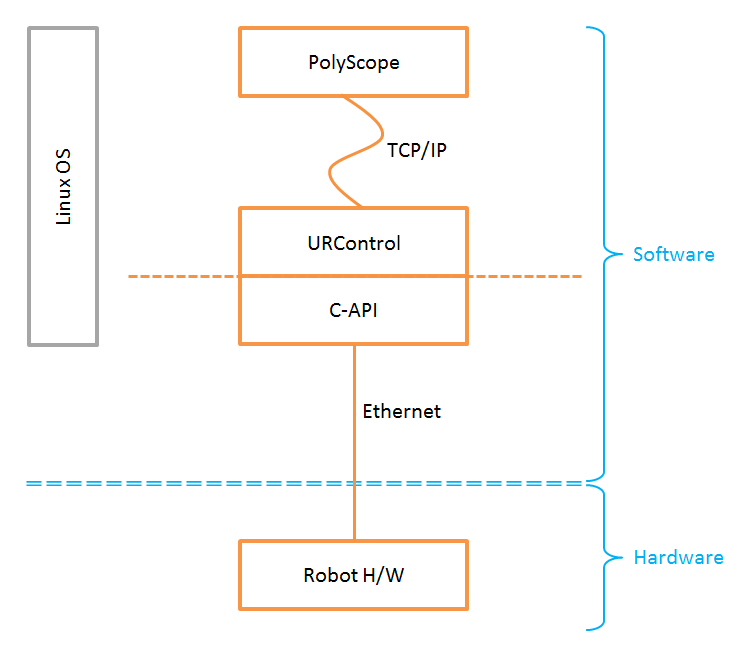
\includegraphics[width=0.8\textwidth]{pic/ur_programming_levels.png}
      \caption[Schichten der Software Schnittstellen]{Übersicht über die
      Schichten der bestehenden Software Schnittstellen des Ur5 Roboters}
      \label{fig:schnittstellen_schichten}
\end{figure}

\section{Kriterien für die Bewertung der Schnittstellen}
\label{sec:criterias_of_solutions_kon}

Die Schnittstellen werden wie folgt bewertet:

\begin{itemize}
\item Programmierbarkeit
\item Interaktion mit Programm,
\item Möglichkeit zu Debuggen und Testbarkeit
\item Aufwendung
\end{itemize}

Wie schwer ist es ein Programm für die einzelnen Schnittsellen zu entwickeln.
Kann der Mensch das Programm Intuitiv bedienen? Wichtig hierbei ist, dass der Mensch mit dem Roboter Kommunizieren kann. Dies geschieht am besten, wenn der Mensch nicht Kryptisch was eingeben muss. Der Mensch braucht Anwenderfreundliche Programme.
\\\\
Beim Entwickeln von Programmen ist es wichtig, dass der Entwickler Fehler im Programm entdeckt um diese schnell zu beheben.
Je Größer und Komplexer das Programm wird, desto schwieriger wird es Fehler zu entdecken.


\section{URControl}
\label{sec:ur_control_gru}

Der URController eine Server Anwendung die auf dem Rechner des Roboters läuft. 
Dieser Controller dient als Schnittstelle von der Roboter Hardware und Software die den Roboter ansteuern wollen.

\subsection{Konfiguration des URControllers}
\label{urcontrol_rci_gru}

Den URController kann man bevor er gestartet wird in einer Konfigurationsdatei konfigurieren.
Hier werden wichtige Einstellungen vorgenommen, die zu den jeweiligen Modellen der Ur5 oder Ur10 Serie gehören. Folgend ist ein ausschnitt der Konfigurationsdatei zu sehen
\\
\begin{lstlisting}
[Config]
# masterboard_version, 0 = Zero-series, 1 = One-series, 
# 3 = Pause function enabled, 4 = first cb2 version, 5 = ur10 support added
masterboard_version = 4
dump_bytecode_on_exception = 1

[Hardware]
controller_box_type = 2 # 1=CB1, 2=CB2UR5, 3=CB2UR10
robot_type = 1  # 1=UR5, 2=UR10
robot_sub_type = 1
\end{lstlisting}

\subsection{Echtzeit Schnittstelle}
\label{urcontrol_rci_gru}

Die Echtzeit Schnittstelle ist eine TCP Schnittstelle, die im 125Hz Takt Nachrichten an die Clients sendet. Diese Schnittstelle empfängt keine Daten von den Clients. Diese Nachrichten müssen von den Clients analysiert und zerlegt werden. Die Daten werden in einer bestimmten form gesendet

TODO !! listing echtzeit schnittstelle

Die Client Anwendung muss nun dieses Packet parsen(Parser: Informationen zerlegen und entsprechend interpretieren.)
Wie Die einzelnen Packete aussehen sind im Anhang mitgeliefert
Für die Programmiersprache C wurde ein ein Parser dafür geschrieben.

\subsection{Secondary und Primary Schnittselle}
\label{urcontrol_spi_gru}

Das Secondary Interface ist eine TCP Schnittstelle, die in einem 60Hz Takt Nachrichten über den Roboter an Verbundene Rechner sendet.
Die Nachrichten beinhalten Informationen wie z.B. den Roboter Status, die Positionen der einzelenen Joints.
Die volle Beschreibung welche Informationen gesendet werden ist im anhang zu finden.

Zusätzlich, kann die Secondary Schnittstelle befehle von Verbundenen Rechnern empfangen. 
Diese Befehle können URScript befehle sein. Ein ganzes Programm aus URScript befehlen oder spezielle zugelassene Befehle die den Roboter Status verändern.

\begin{figure}[ht]
  \centering
    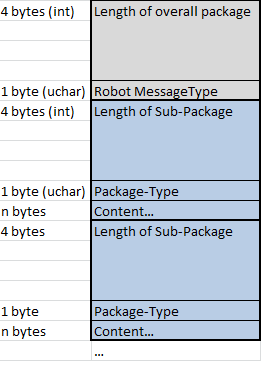
\includegraphics[width=0.5\textwidth]{pic/secondary_datapackage_scheme.png}
      \caption[Schema des Datenpackets gesendet von der Secondary Schnittstelle]{Grobe Darstellung wie das Nachrichten Packet gesendet von der Secondary/Primary Schnittstelle.}
      \label{fig:datascheme_of_secondary_interface}
\end{figure}

\subsection{Polyscope}
\label{urcontrol_polyscope_gru}

Polyscope ist eine Anwendung die auf dem Roboter-Rechner läuft. Die Anwendung verbindet sich per TCP/IP auf den UR Controller und sendet URScript befehler an den Roboter um diesen zu steuern.
Diese Anwendung wird auf dem Tablet angezeigt. Hierrüber kann man per Touch eingabe ein neues .URP Programm erstellen. Dieses Programm wird zur Laufzeit in ein .script umgewandelt.

\section{C-API}
\label{sec:rest_prinzip_gru}

Die C-API ist von dem Hersteller UR eine zur Verfügung gestellte C Library mit einer Header Datei, die etwaige Funktionen der Library erklärt. Die Header Datei enthält nicht alle Funktionen, somit sind nicht alle zugänglich. Die C-API erlaubt es einen eigenen Controller für den Roboter zu entwickeln. Der für den Roboter zur Verfügung gestellte Controller mit der Polyscope Software können aber nicht gleichzeitig laufen. Es schließen sich also die URScriptsprache und ein eigener Controller zunächst aus. Es könnte ein eigener Controller gebaut werden der die Befehle in URScript selbst interpretiert und diese wie bei dem URController ausführt. So könnte man die vorhandene Sprache nehmen und diese sogar erweitern.

\subsection{Kontrollstruktur}
\label{capi_control_loop_gru}	

Die C-API ermöglicht es eine Verbindung zum Roboter zu öffnen und über eigene Funktionen Befehle abzuschicken. Dies erfolgt in einem streng festgelegten Muster. Dieses Muster ist in Abbildung ... TODO !! abilbundsref zu sehen. 
die Funktion robotinterface\_read\_state\_blocking() startet den Bereich in dem Datenabfragen an den Roboter gestellt werden können. Daten wie zb. Temperatur der Motoren, der Stand der Gelenke, die Geschwindigkeit der Gelenke, etc. in der Dokumentation beiliegend zu dieser Arbeit sind alle Daten noch einmal aufgelistet. Nachdem die Daten abgefragt werden, kann mit C-API Functionen Position, Geschwindigkeit und Beschleunigungswerte übermittelt werden, die der Roboter durch seinen Regler auszuführen versucht.\\
Es können jedoch keine Wegpunkte festgelegt werden, die dann automatisch vom Roboter angefahren werden. Dies muss der Entwickler selbst 
berechnen. Es gibt mehrere Verfahren, in dieser Arbeit sind PTP-Verfahren(sieht Kapitel \ref{ptp_capi_gru}) und Linear Verfarhen(siehe Kapitel \ref{linear_capi_gru}) getestet worden. In der beiliegenden Dokumentation ist aufgeführt wie man dies möglicherweise berwerkstelligen könnte.
\\\\
Zum Abschluss wird die Function robotinterface\_send() aufgerufen die dafür sorgt, dass der Acht millisekundentakt eingehalten wird und die Befehle an den Roboter weiterleitet. Falls die Acht Millisekunden überschritten werden, wird der Roboter in einen Sicherheitsmodus gesetzt
und der Roboter wird angehalten.\\
Wenn so etwas im UR-Kontroller passiert, kann der Anwender diese wieder abschalten wenn alles in Ordnung ist. Dies muss mit der C-API selbst geschrieben werden. Die API liefert hierfür auch funktionen. Das die richtigen Richtlinien aber auch eingehalten werden, muss von dem wechsel des Sicherheitsmodus in den normalen Modus eine Benutzerabfrage verlangt werden.

\subsection{PTP Verfahren}
\label{ptp_capi_gru}

Um den Roboter bestimmten Wegpunkten abfahren zu lassen, muss man die Bewegungsprofile selbst berechnen und ǘber die C-API an den Roboter im 125Hz Takt übergeben. Das PTP Verfahren setzt dabei vorraus das die einzelnen Positionen der Gelenke bekannt sind. Der Wert ist angegeben in radiant. Die Zielposition

\subsection{Linear Verfahren}
\label{linear_capi_gru}

Das Lineare Verfahren bedeutet eine Bewegung des Roboters von dem TCP Punkt aus. Sie verfährt Linear, bedeutet das die Orientierung 
des TCP Punktes sich nicht ändert. Da in diesem Verfahren die Berechnung der Position des TCP Punktes verwendet wird, ist es nötig die Position des TCP im Raum zu kennen um eine Strecke zu einem Ziel Punkt abfahren zu können. Der Roboter kann aber nur Positionen die der Sechs Gelenke verarbeiten. Es muss also eine umrechnung stattfinden. Diese umrechung wird Inverse Kinematic genannt. Die Berechnung für die Ineverse Kinematic ist von einem anderen Projekt entnommen worden.
 \chapter{Konzept}
\label{konzept_kon}
Lorem ipsum dolor sit amet, consetetur sadipscing elitr, sed diam nonumy eirmod tempor invidunt ut labore et dolore magna aliquyam erat, sed diam voluptua. At vero eos et accusam et justo duo dolores et ea rebum. Stet clita kasd gubergren, no sea takimata sanctus est Lorem ipsum dolor sit amet. Lorem ipsum dolor sit amet, consetetur sadipscing elitr, sed diam nonumy eirmod tempor invidunt ut labore et dolore magna aliquyam erat, sed diam voluptua. At vero eos et accusam et justo duo dolores et ea rebum. Stet clita kasd gubergren, no sea takimata sanctus est Lorem ipsum dolor sit amet.

\section{Anwendungsbeispiel}
\label{sec:anwendung_kon}

Das Anwendungsbeispiel ist ein Kinderspiel. Dieses Spiel soll die motorischen Fähigkeiten bei Kindern verbessern.
Gegeben ist ein Kugel mit löschern aus Verschiedenen Formen(Kreis, Oval, Viereck, Trapez, etc.). Zu diesen Formen existieren die Entsprechenden Klötzchen, die entsprechend Groß sind un die Form der Löscher besitzen. Die Aufgabe des Spiel ist es alle Klötzchen in die entsprechende Form zu drücken, bis alle in der Kugel sind.
\\
Die Kugel wird an den Kopf des Roboterarms befestigt. Es soll eine Anwendung entwickelt werden, die für den entsprechenden Spieler die Höhe des Roboters einstellt. Der Spieler soll die möglichkeit haben diese Start Position zu verstellen und für sich zu speichern. Bei einem bestimmten Knopf druck soll der Roboter das Loch für die jeweils nächste Form so ausrichten, damit der Mensch das Klötzchen nurnoch einwerfen braucht.

\section{Speichern der Anwendungsdaten}
\label{sec:save_of_data_kon}

Um Auf bestimmte Menschen zugeschnittene Bewegungsabläufe zu machen muss der Roboter Daten über den Anwender kennen. Diese sollten persistent gespeichert werden, damit bei einem wechsel des Anwenders die Daten nicht verloren gehen.
Daten der Anwender sind z.B Name, Alter, bestimmte Positionen im RoboterProgramm, etc.

\subsection{Speichern über Polyscope und URScript}
\label{sec:save_data_polyscope_kon}

In der Polyscope Software oder in einem URScript Programm, können Daten die von den Benutzern erstellt oder erhoben werden nicht persistent
gespeichert werden. Hierzu muss eine Zweite Anwendung Entwickelt werden, auf die sich das URScript oder URP Programm verbindet und die Daten zum persistenten speichern versendet.
\\
In Polyscope und URScript muss sehr aufwendig mit den vorhandenen Script Befehlen eine Socket Verbindung aufgebaut werden.
Damit diese Zwei Programme miteinander Kommunizieren können muss ein gemeinsames Protokoll mit bestimmten Befehlen festgelegt werden.

\subsection{Speichern über Eigene API}
\label{save_data_own_api_kon}

Mit der Eigenen API muss keine zweite Software entwickelt werden, da die API auf einem Client Rechner läuft und dort die Daten persistent gespeichert werden können. Es muss im Anwendungsprogramm eine verbindung zu einer Datenbank aufgebaut werden und dort können die Daten gespeichert werden.
 \chapter{Realisierung}
\label{chap:umsetzung}

\section{C-API}
\label{sec:capi_rel}

In folgendem Kapitel wird beschrieben wie die C-API genutzt werden kann, um den Roboter bestimmte Wegpunkte abfahren zu lassen.

\subsection{Beispielanwendung}
\label{sub:capi-problems_rel}

Es konnte eine Anwendung erstellt werden, die den Roboter initialisiert und dann in einer Schleife die Positions-, Geschwindigkeits-und Beschleunigungsdaten sendet. Des weiteren konnte ein Bewegungsprofil errechnet werden, dem der Roboter gefolgt ist.
\\\\
Bevor man Daten vom Roboter abfragen kann, muss eine Verbindung zum Roboter hergestellt werden, ihn mit Strom versorgen und initialisieren lassen. Folgend werden diese Vorgänge beschrieben.\\
Mit dem Befehl \sona{robotinterface\_open()} kann die Verbindung zum Roboter hergestellt werden.
\\\\
Um sicherzugehen, dass die Verbindung offen ist, wird wiederholend in einer Zeitspanne, immer wieder abgefragt, ob der Roboter verbunden ist. Falls dies nicht funktioniert, wird der Vorgang abgebrochen und das Programm sollte beendet werden. Es kommt vor, dass der Roboter beim Starten noch in einem Sicherheitsmodus ist. Wenn dies der Fall ist, muss der Modus abgestellt werden. Dies geht mit der Funktion \sona{robotinterface\_unlock\_security\_stop();}.
\\\\
Auch hier wird zur Sicherheit, der Befehl wiederholt an den Roboter gesandt. Wenn der Roboter dennoch im Sicherheitsmodus bleibt, ist es möglich, dass der Notausschalter am Touch Tablet aktiviert ist.
\\
Nachdem die Verbindung offen ist, muss der Roboter mit Strom versorgt werden. Mit dem Befehl \sona{robotinterface\_power\_on\_robot()} kann das bewerkstelligt werden. Auch hier wird wiederholend gewartet und abgefragt, bis der Roboter hochgefahren ist. Ob der Roboter hochgefahren ist, kann mit der Funktion \sona{robotinterface\_is\_power\_on\_robot()} abgefragt werden.
\\\\
Nun wird der Roboter initialisiert. Er geht nach dem Starten automatisch in den Initialisierungs-Modus. Jedes einzelne Gelenk muss nun so lange in eine Richtung bewegt werden, bis das Gelenk in den normalen Modus übergeht. Um die Gelenke zu bewegen, wird eine Geschwindigkeitsvorgabe an den Roboter gesandt. (siehe Listing \ref{lst:initialize_robot_lst})

\begin{lstlisting}[language=C,caption={Initialisierung der einzelnen Gelenke}, label=lst:initialize_robot_lst,captionpos=b]
puts("Initializing robot");
/// Set zero velocity and acceleration as guard
int j;
for (j=0; j<6; ++j) {
  pva_packet.velocity[j] = 0.0;
  pva_packet.acceleration[j] = 0.0;
}
do {
  ++i;
  robotinterface_read_state_blocking();
  int j;
  for (j=0; j<6; ++j) {
    // initialize_direction is 1 or -1. it determines in which direction die Joint is moving during the initialization
    pva_packet.velocity[j] = ((robotinterface_get_joint_mode(j) == JOINT_INITIALISATION_MODE)) ? (initialize_direction)* 0.1 : 0.0;
   }
  robotinterface_command_velocity(pva_packet.velocity);
  robotinterface_send();
} while (robotinterface_get_robot_mode() == ROBOT_INITIALIZING_MODE && exit_flag == false);
puts(" Done!");
\end{lstlisting}

Nachdem die Initialisierung abgeschlossen ist, muss wie in Listing \ref{lst:robot_control_loop} eine Schleife mit der vorgegebenen Struktur durchlaufen werden, bis das Programm beendet, oder die Verbindung zum Roboter geschlossen werden soll. Wenn dies nicht so gehandhabt wird, geht der Roboter automatisch in den Sicherheitsstopp, da nicht innerhalb von acht Millisekunden Nachrichten an den Roboter gesendet wurden.
\\\\
Innerhalb der beiden Befehle \sona{robotinterface\_read\_state\_blocking()} und \sona{robotinterface\_send()} kann nun eine Interpolation berechnet werden und die Vorgaben für Position, Geschwindigkeit und Beschleunigung an den Roboter gesandt werden(siehe Listing \ref{lst:interpolate}).

\begin{lstlisting}[language=C,caption={Interpolation eines berechneten Wegs}, label=lst:interpolate,captionpos=b]
// loop through interpolation length  
for(i=0; i < move_pva_packet.interpolations+1; i++){
  robotinterface_read_state_blocking();

  // abort interpolation if Robot is in securitystop mode
  if(robotinterface_is_security_stopped()) {
      robotinterface_get_actual_current(currents_actual);
      robotinterface_command_empty_command();
      robotinterface_send();
      break;
  }

  // get current time of interpolation 
  move_pva_packet.point_in_time= (double) i * T_IPO;

  // interpolate with sinoide profile and write result in variable move_pva_packet
  interpolation_sin_ptp(&move_pva_packet);

  // write the triple to robot
  robotinterface_command_position_velocity_acceleration(move_pva_packet.pva.position,
                                                        move_pva_packet.pva.velocity,
                                                        move_pva_packet.pva.acceleration);
  // send command to robot
  robotinterface_send();
}
\end{lstlisting}

\subsection{Bewegungsprofil berechnen und interpolieren}
\label{sub:profile_and_interpolation_rel}

Ein Bewegungsprofil besteht aus 3 Phasen: Beschleunigungs-, Konstantfahrt-und Bremsphase.
Die Formeln für die Berechnung sind dem Buch ``Industrieroboter: Methoden der Steuerung und Regelung'' \cite{WW-2013} entnommen.
\\
Eine sanfte Beschleunigung schont die Robotergelenke. Dies wird auch Sinoidenprofil genannt. Die Formeln in der Lektüre können einfach übernommen und müssen nur ausprogrammiert werden. In der Dokumentation ist die Interpolation und Berechnung für eine PTP-und Linear-Bahn
genau beschrieben.
\\\\
Um die Berechnung des Profils zu testen, kann simuliert interpoliert werden und die einzelnen Angaben in den Interpolationsschritten geloggt werden. Nachher werden die geloggten Daten in Matlab\footnote{``MATLAB® ist eine höhere Programmiersprache und interaktive Umgebung für numerische Berechnungen, Visualisierung und Programmierung. MATLAB dient zur Datenanalyse, Algorithmen-Entwicklung und zur Erstellung von Modellen und Anwendungen.''\cite{MATLAB-2014}} geplottet.
Folgend sind die Profile der Positions-, Beschleunigungs-und Geschwindigkeitswerte für eine PTP-Bahn geplottet.

\begin{figure}[H]
  \centering
    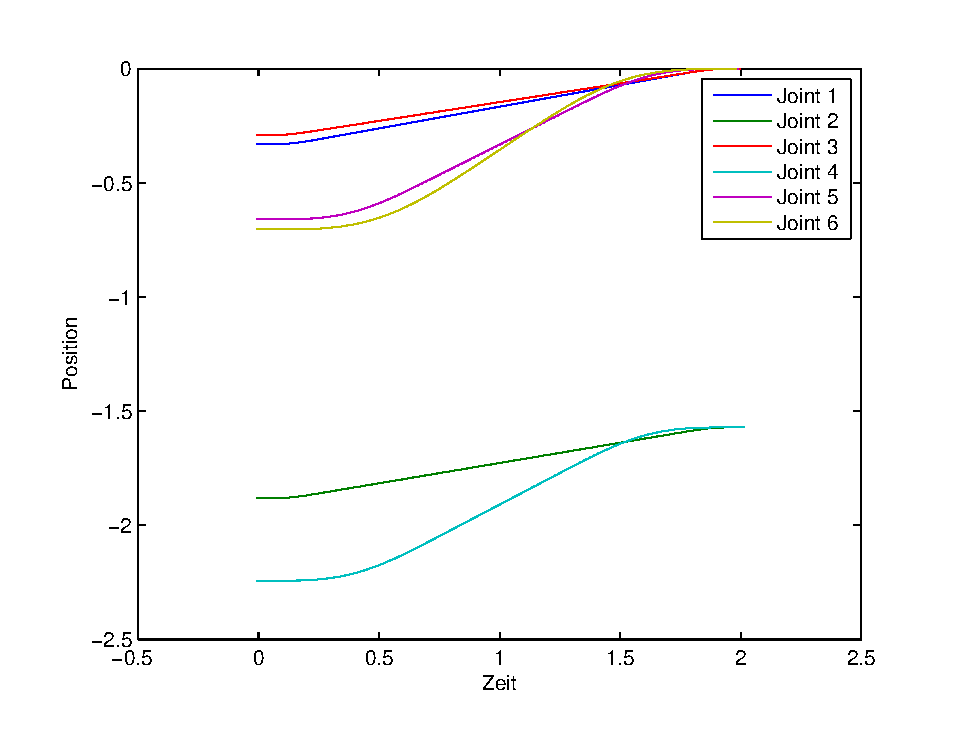
\includegraphics[width=0.8\textwidth]{pic/position_profile.eps}
      \caption[Positionsprofil einer PTP-Bahn in Matlab gepplotet]{Die Abbildung zeigt das Positionsprofil einer PTP-Bahn mit allen Gelenken. Position ist angegeben in Radiant.}
      \label{fig:position_ptp_profile}
\end{figure}

\begin{figure}[H]
  \centering
    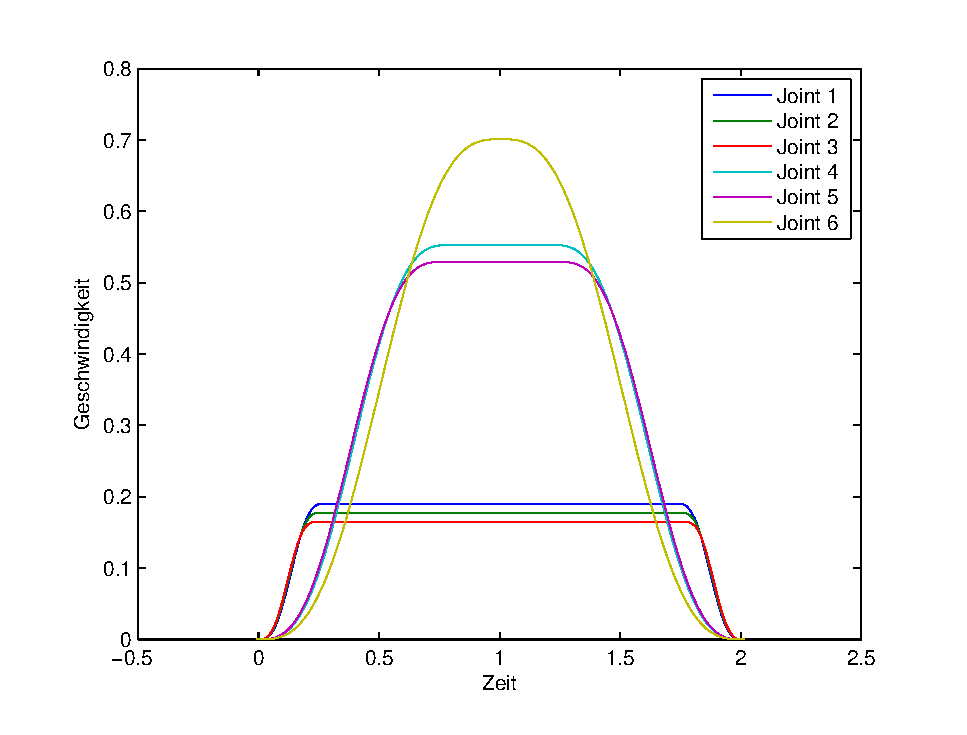
\includegraphics[width=0.8\textwidth]{pic/velocity_profile.eps}
      \caption[Geschwindigkeitsprofil einer PTP-Bahn in Matlab gepplotet]{Die Abbildung zeigt das Geschwindigkeitsprofil einer PTP-Bahn mit allen Gelenken. Die Geschwindigkeit ist angegeben in Radiant/Sekunde.}
      \label{fig:velocity_ptp_profile}
\end{figure}

\begin{figure}[H]
  \centering
    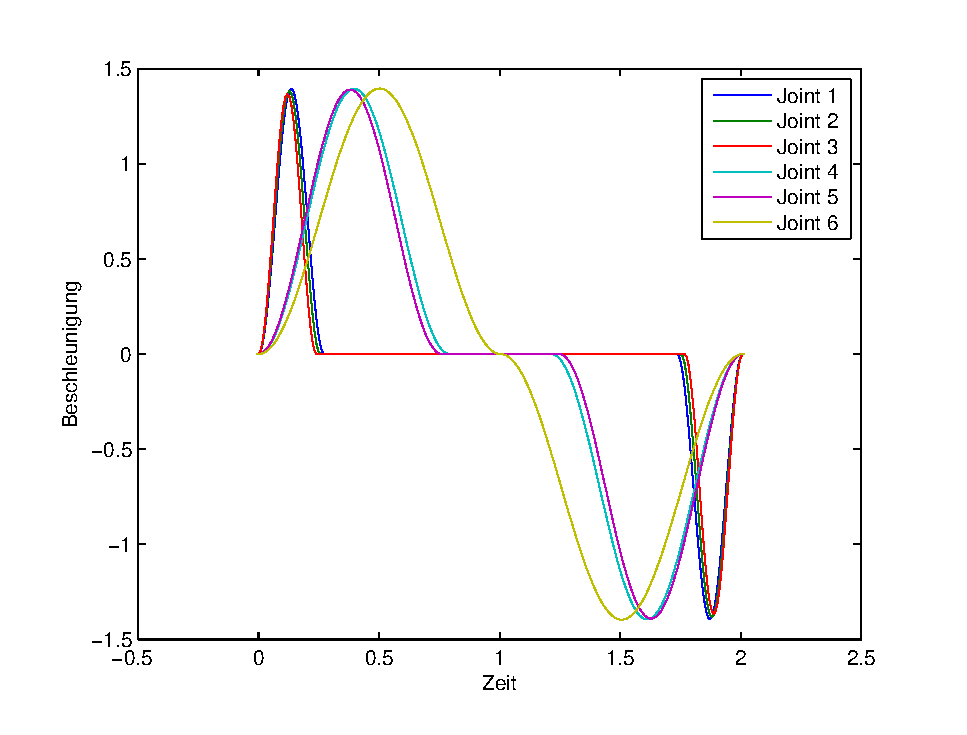
\includegraphics[width=0.8\textwidth]{pic/acceleration_profile.eps}
      \caption[Beschleunigungsprofil einer PTP-Bahn in Matlab geplottet]{Die Abbildung zeigt das Beschleunigungsprofil einer PTP-Bahn mit allen Gelenken. Die Beschleunigung ist angegeben in Radiant/Sekunde²}
      \label{fig:acceleration_ptp_profile}
\end{figure}

\subsection{Aufgetretene Probleme}
\label{sub:capi-problems_rel}

Der Roboter geht ab einem bestimmten Winkel in den Sicherheitsstopp. Die Abweichung der Position wird zu groß. Dies kann analysiert werden, wenn man sich den Durchschnitt der Soll-und Ist-Werte der Position ansieht (siehe Abbildung \ref{fig:position_join1}). Es ist deutlich zu erkennen, dass die Abweichung beim 2. Gelenk steigt. Die Motorleistung reicht anscheinend nicht aus, um über die Schwelle der Reibungskräfte und die Erdanziehung zu kommen. Zu sehen ist in Abbildung \ref{fig:joint_1_position_capi}, dass für die Stromstärke ein Offset mitberechnet wird. Vergleicht man die Werte, die bei derselben Bewegung von Polyscope berechnet werden (siehe Abbildung \ref{fig:current_profile_joint1_rci}), sieht man eine höhere Stromstärke bei der Polyscope Software, bei der die Bewegung ohne Probleme funktioniert.
\\
\begin{figure}[H]
  \centering
    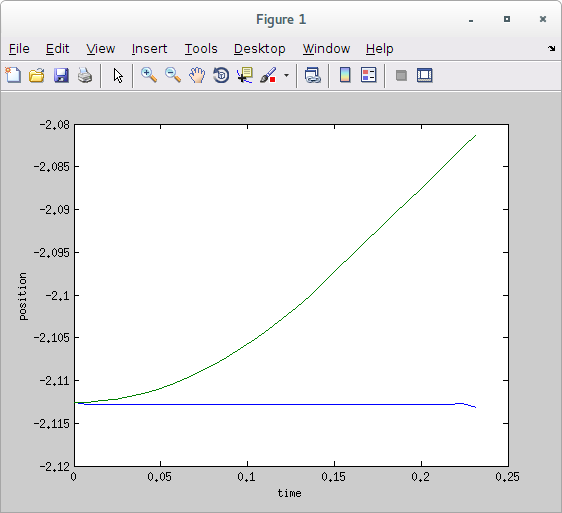
\includegraphics[width=0.6\textwidth]{pic/joint1_position_capi.png}
      \caption[Soll-und Ist-Werte der Position]{Abbildung zeigt die Soll-und Ist-Werte der Position bis zum Sicherheitsstop des Roboters}
      \label{fig:position_join1}
\end{figure}

Mit der C-API ist es nicht möglich, selbst den Wert der Stromstärke vorzugeben, deswegen sind die Soll-Werte bei der Polyscope Software und der eigenen Anwendung mit der C-API etwas verschieden.
\\
Bei dem 2. Gelenk ist auch zu beobachten, dass dieses nicht rechtzeitig anhält, wenn der Notausschalter betätigt wird. Bei einem solchen Versuch ist der Roboter zu spät angehalten. Deswegen ist auch eventuell von einem Hardwaredefekt auzugehen.

\begin{figure}[H]
  \centering
    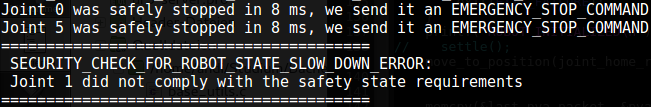
\includegraphics[width=0.8\textwidth]{pic/emergency_stop_capi.png}
      \caption[Warnungsausgabe für 2. Gelenk nach Notausschalter]{Abbildung zeigt eine Warnung die von der C-\ac{API} ausging, weil das 2.Gelenk nicht rechtzeitig nach einem Notaus angehalten hat}
      \label{fig:acceleration_ptp_profile}
\end{figure}
\newpage
\section{Polyscope}
\label{sec:Polyscope_rel}

\subsection{Programmierung}
\label{sub:programmierung_polyscope_rel}

Die Programmierung findet meist nur auf dem Touch Tablet statt. Ein neues Programm fängt mit einem leeren Ereignisbaum an. Es können per Toucheingabe alle möglichen Funktionen, die die Script Sprache bietet, dem Ereignisbaum hinzugefügt werden. Wenn das Programm abläuft, werden von der Wurzel an die Befehle abgearbeitet.
Wie in Abbildung \ref{fig:programm_in_polyscope} zu sehen ist, ist die Ansicht des Programmbaumes sehr unübersichtlich.

\begin{figure}[H]
  \centering
    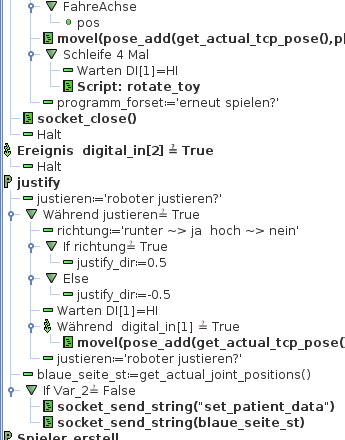
\includegraphics[width=0.5\textwidth]{pic/polyscope_program_tree.png}
      \caption[Programm Baum in Polyscope]{Ein Ausschnitt aus einem Programm Baum in Polyscope}
      \label{fig:programm_in_polyscope}
\end{figure}

Es ist möglich, andere Script Dateien in das Programm einzufügen. Dazu gibt es das Feld \sona{Script}. Das Script-Programm muss sich auf dem Linux-Rechner befinden. Man muss daher das Script Programm auf einem anderen Rechner programmieren und bei jeder Änderung auf den Linux-Rechner des Roboters senden. Mit dieser Möglichtkeit könnten Programmabschnitte ausgelagert werden. Es ist aber nicht ersichtlich, welche Script Dateien benutzt werden.\\
Alternativ zum Touch Tablet, könnte der X-Server von dem Linux-Rechner auf einen anderen Rechner umgeleitet werden, um dort mit dem Programm per Maus und Tastatur zu arbeiten. Dies wurde aber noch nicht getestet und es könnte zu Verzögerungen beim Ausführen kommen.
\\
Eine andere Möglichkeit, ein Programm unter Polyscope zu programmieren, gibt es nicht.

\subsection{Benutzer-Interaktion}
\label{user_interaktion_polyscope_rel}

Die Möglichkeiten zur Interaktion mit dem Benutzer sind sehr begrenzt. Die Software und die URScript Sprache lassen es zu, dass auf dem Touch Tablet Popups auftauchen. Wenn man mit dem Benutzer interagieren will, gibt es mehrere Arten dieser Popups.
Als Nachricht, ja/nein Fragen, oder Text abfragen. Der Benutzer kann dann mit einem Text antworten oder klickt auf einen Ja-bzw. Nein-Button. In Abbildung \ref{fig:polyscope_popup} ist als Beispiel eine Nachricht und ein Ja/Nein Popup zu sehen.

\begin{figure}[H]
  \centering
    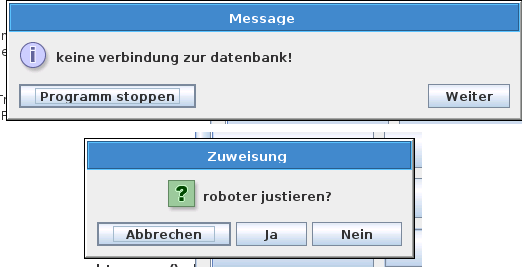
\includegraphics[width=0.8\textwidth]{pic/popup_question.png}
      \caption[Popup in Polyscope]{Abbildung zeigt zwei verschiedene Arten von Popups in Polyscope}
      \label{fig:polyscope_popup}
\end{figure}

Kompliziertere Menüs sind mit dieser Methode nicht möglich. Wenn ein Programm erstellt werden soll, bei dem der Benutzer viele Eingaben machen muss, lässt sich das mit Polyscope nur sehr schwer realisieren.

\subsection{Test und Fehlersuche im Programm}
\label{debuggin_polyscope_rel}

Bevor Polyscope ein Programm ablaufen lässt, wird das Script auf die richtige Syntax geprüft. Sollte ein Fehler vorhanden sein, wird dies beim Start als Popup angezeigt. Fehler, die in Abschnitten mit Touch hinzugefügt wurden, können jedoch nicht lokalisiert werden. Nur in extra eingefügtem Script Code kann grob lokalisiert werden, welcher Fehler aufgetreten ist, weil dieser Teil extra geprüft wird.
\\\\
Da das Programm mit dem Touch Tablet ausgeführt werden kann, kann man während der Programmierung das Programm kurz ablaufen lassen um zu Testen. So kann sehr schnell getestet werden ob die gewünschten Einstellungen dem Ergebnis entsprechen. Bei großen Programmen mit vielen Benutzeranfragen, kann dies jedoch viel Zeit in Anspruch nehmen. Es muss von einem Benutzer bei jeder Anfrage eines Popups von Hand geantwortet werden.

\subsection{Aufwand der Programmierung}
\label{polyscope_aufwand}

Kleine Programme in Polyscope sind schnell geschrieben. Mit dem Touch Tablet kann rapide eine kleine Kontrollstruktur aufgebaut werden. Das Tablet hat jedoch große Nachteile. Wie in Abbildung \ref{fig:programm_in_polyscope} zu sehen ist der Bereich für den Ereignisbaum äußerst klein. Wenn ein Programm nun z. B. 500 Befehle enthält, ist es nicht möglich den Überblick zu behalten. Außerdem ist es ziemlich aufwändig, zwischen bestimmten Bereichen hin und her zu wechseln, da das Touch Tablet nicht genau ist. Es ist möglich, größere Bereiche auf Scirpt Dateien auszulagern, um diese dann im \ac{URP} zu verwenden. Das erlaubt die Wiederverwendung von Code. Mit dem Touch Tablet ist es jedoch nicht angenehm, diese zu programmieren und anzupassen.

\subsection{\ac{TCP/IP} Server mit Datenbank zum dauerhaften Speichern der Daten}
\label{tcp_datentank_sicherung_rel}

Um mit Polyscope und URScript erhobene Daten zu speichern, wurde ein kleiner \ac{TCP/IP} Server geschrieben, der eine Verbindung zulässt und Daten in einer Datenbank speichert. Die Daten sind objektorientiert, und werden von dem Server erstellt.
In Polyscope und URScript gibt es keine Objektorientierung, deshalb muss dort alles nacheinander abgefragt werden.
Ein Beispiel einer \ac{TCP/IP} Servers ist im Anhang aufgeführt (siehe \ref{save_data_tcp_code_gru}).

\section{URScript}
\label{sec:ur_script_rel}

Die URScript Sprache ist sehr stark an Python gelehnt.
Das Manual von Univeral Robots umfasst alle nötigen Funktionen, um komplexe Aufgaben zu erfüllen.
Um Daten persistent zu speichern, muss wie in Polyscope eine Socket-Verbindung zu einer zweiten Anwendung aufgebaut werden, die die Daten speichert (siehe \ref{tcp_datentank_sicherung_rel})

\subsection{Laden des Scripts auf den Controller}
\label{load_script_rel}

Das Script kann nicht direkt auf dem Rechner über die Polyscope Software ausgeführt werden. Um ein selbst geschriebenes Programm in URScript auszuführen, ist es von nöten, sich mit der Secondary Schnittstelle des URControllers \ref{urcontrol_spi_gru} per \ac{TCP/IP} zu verbinden und dann die einzelnen Zeilen der Script Datei an den Controller zu senden.
\\\\
Es ist möglich, einzelne Befehle oder ein großes Programm auszuführen. Um einzelne Befehle auszuführen, werden diese nacheinander versendet.
Ein ganzes Programm wird versendet, indem, wie in Listing \ref{lst:urscipt_program_lst} gezeigt, eine Funktion die ganzen Befehle umschließt. Der Controller führt diese Funktion aus, sobald diese mit dem ``end'' der Funktion abgeschlossen ist.
Zu beachten ist noch, dass der URController am Ende jeden Befehls oder Programms einen Zeilenumbruch erwartet.

\begin{lstlisting}[caption={Kleines Beispielprogramm in URScript}, label=lst:urscipt_program_lst ,captionpos=b] 
def myProg():
	popup("hello world","test", False, False)
	set_digital_out(1, True)
	movej([0.23,1.23,0.343,0.34.0.0,0.0],a=0.5,v=0.3)
end
\end{lstlisting}

\subsection{Programmierung}
\label{programmierung_ur_script_rel}

Programmiert werden kann das Script mit allen vorhandenen Textverarbeitungsprogrammen. Vorteilhaft ist es, wenn das Programm Syntax Highlighting\footnote{Zur Verbesserung der Lesbarkeit und der Übersicht, wird in einem Textverarbeitungsprogramm der Programmcode unterschiedlich dargestellt. Meist mit unterschiedlichen Farbwerten. Der Entwickler sieht mit einem Blick, ob er es mit Textvariablen oder Zahlenwerten zu tun hat.} für Python beherrscht. Da URScript ja sehr stark an Python angelehnt ist, trägt dieses Verfahren zu einem besseren Überblick bei.
\\\\
Die Sprache bietet keine Möglichkeiten, Kommentare zu nutzen, was aber sehr wichtig ist, wenn ein Programm wächst und mehrere Programmierer am Projekt beteiligt sind. Es ist wichtig für die Verständlichkeit. Deshalb wurde dafür in dem Programm, welches das URScript liest und an die Schnittstelle sendet, ein Pre-Prozessor eingebaut. Die Script Datei wird nach Kommentaren durchsucht und schneidet diese vor dem Senden heraus. (siehe \ref{lst:urscipt_comment_lst}).

\begin{lstlisting}[caption={Beispiel-Kommentare vor und nach dem Pre-Prozessor}, label=lst:urscipt_comment_lst ,captionpos=b]
  def testprog():
    # mit # wird ein Kommentar angefangen
    movej([0.23,1.23,0.343,0.34.0.0,0.0],a=0.5,v=0.3) # Bewegung auf Achs Ebene zur Startposition
  end

  wird zu 

  def testprog():
    movej([0.23,1.23,0.343,0.34.0.0,0.0],a=0.5,v=0.3)
  end

\end{lstlisting}

\subsection{Test und Fehlersuche im Programm}
\label{ur_script_debuggen}

Nach dem Senden des Programms an den URController ist die einzige Möglichkeit, zu sehen ob das Programm Fehler enthält, wenn der Controller ein entsprechendes Bit setzt, das in den Datenpaketen von der Secondary Schnittstelle gesendet wird. Über dieses ``Programm läuft'' Bit, kann man sehen ob ein Programm läuft oder nicht.
\\
Wenn das Script Programm nicht abläuft, erhält man keinerlei Fehlermeldungen. Um Fehler auszuschließen, muss also der Bereich isoliert werden, in dem der Fehler vorkommt. Das geht meist nur in einem aufwändigem Ausschlussverfahren, bei dem immer wieder Script Code entfernt wird.

\subsection{Benutzer Interaktion}
\label{ur_script_user_interaction}

Das Manual für URScript nennt nur die Popup-Funktion, um dem Anwender eine Nachricht zu geben. Andere Möglichkeiten zur Interaktion sind im Manual nicht angegeben. Jedoch bietet Polyscope auch über verschiedene Popup-Arten Möglichkeiten zur Interaktion. Diese Popups gibt es auch für URScript. Die Befehle können aus dem von Polyscope erzeugtem URScript Code von \ac{URP}s eingesehen werden. Somit bestehen genau die gleichen Möglichkeiten wie bei Polyscope.

\subsection{Aufwand der Programmierung}
\label{ur_script_aufwand}

Im Gegensatz zur Polyscope Software, kann mit einem Textverarbeitungsprogramm schnell mit guter Übersicht ein größeres, komplexeres Programm erstellt werden. Es können problemlos mit dem Pre-Prozessor Kommentare eingefügt werden und der Code ist im späteren Fall leichter verständlich für neue Programmierer. Da schwer Fehler zu entdecken sind und deswegen häufig das Programm manuell getestet werden muss, ist dennoch bei umfassenden Anwendungen ein größerer zeitlicher Aufwand von Nöten.

\section{Anwendung mit Adapter zu URScript}
\label{sec:script_hoerherer_schicht_rel}

Im folgenden Kapitel wird das Anwendungsbeispiel in Python entwickelt. Um zu zeigen, wie die Benutzerinteraktion mit einem eigenen Adapter gestaltet werden kann, wurde hierfür die Software Bibliothek \sona{TKinter}\footnote{Mehr Informationen über TKinter unter folgender Website: \url{https://wiki.python.org/moin/TkInter}}, mit der man schnell eine \ac{GUI} entwickeln kann. Die Interaktion erfolgt durch Buttons, die dann über den Adapter Befehle an den Roboter sendet.

\subsection{Adapter zur Secondary Schnittstelle}
\label{beschreibung_script_hoeher_schicht}

Die Scriptbefehle zur Secondary Schnittstelle werden als Text übergeben. Der Adapter wird in Form einer Klasse geschrieben, die die einzelnen Script Befehle in Funktionen mitliefert(siehe Listing \ref{lst:secondary_interface_scriptfunctions}).

\begin{lstlisting}[caption={Ausschnitt zeigt Funktionen, die Scriptbefehle in der Adapter-Klasse umsetzt}, label=lst:secondary_interface_scriptfunctions ,captionpos=b]

# moveJ moves the Robot with joint coordinates
# positions should include the target joint positions
def movej(self, positions=None, a_max=None, v_max=None):
    if positions is None:
        positions= self.get_joint_positions()
    if a_max is None:
        a_max=math.radians(40)
    if v_max is None:
        v_max=math.radians(60)
    message="""movej(%s,a=%f,v=%f)
    """%(positions,a_max,v_max)
    print message
    self.start_program(message)

# movel moves the Robot Linear in kartesian coordinates
# positions should contain the target tcp positions
def movel(self, positions=None, a_max=None, v_max=None):
    if positions is None:
        positions= self.get_tcp_positions()
    if a_max is None:
        a_max=math.radians(40)
    if v_max is None:
        v_max=math.radians(60)
    message="""movel(p%s,a=%f,v=%f)
    """%(positions, a_max, v_max)
    print message
    self.start_program(message)
\end{lstlisting}

Diese Klasse öffnet zwei Verbindungen zur Secondary Schnittstelle. Eine zum Empfangen der Datenpakete und eine zum Senden der URScript Befehle. Der Adapter besitzt eine Queue\footnote{Eine Warteschlange, ähnlich wie bei einem Supermarkt. Die Elemente in einer Queue werden nacheinander abgearbeitet.}, um die Befehle nacheinander zur Secondary Schnittstelle zu senden. Da Befehle eventuell viel Zeit benötigen, um ausgeführt zu werden, wird gewartet, bis der Befehl abgearbeitet oder abgebrochen wurde. Erst dann wird in der Queue der nächste Befehl an die Schnittstelle gesendet.

\begin{lstlisting}[caption={Ausschnitt zeigt die Abarbeitung der Queue}, label=lst:adapter_queue ,captionpos=b] 
while self.__run_flag:
    DequePrograms.lock.acquire()
    if(len(self.s_interface.program_queue) > 0):
        # print("message queue contains messsages %d" % len(self.s_interface.program_queue))
        message=self.s_interface.program_queue.popleft()
    else:
        message=None
    DequePrograms.lock.release()
    if(message is not None):
        SecondSendInterface.send_lock.acquire()
        self.s_interface.send_messages_queue.append(message)
        SecondSendInterface.send_lock.release()

        //blocks the thread until URScript finishes
        self.s_interface.block_program()
    time.sleep(0.2)
return 0
\end{lstlisting}

In einer Anwendung kann nun diese Klasse benutzt werden, um den Roboter zu steuern.
Der Aufwand für ein Programm ist mit einer eigenen API anfangs deutlich höher als die URScript-Sprache direkt zu nutzen. Es muss erst ein Adapter geschrieben und getestet werden, bevor die eigentliche Anwendung geschrieben werden kann. 

\subsection{Programmierung mit Adapter}
\label{programmierung_mit_hoerherer_schicht}

Sobald der Adapter in einer etablierten Programmiersprache programmiert ist und Fehler in diesem so gut wie ausgeschlossen sind, kann nun mit normalen Softwareentwicklungstechniken leicht ein Programm geschrieben werden. In dieser Arbeit wurde Python gewählt. Python bietet viele Bibliotheken und Design Patterns, die das Programmieren vereinfachen. Es können Entwicklungswerkzeuge benutzt werden, um einen guten Überblick über das Programm zu behalten.

\subsection{Benutzer-Interaktion}
\label{user_interaktion_mit_hoerherer_schicht}

Eine etablierte Programmiersprache bietet natürlich verschiedene Bibliotheken und Möglichkeiten, ein interaktives und leicht verständliches Interface zu erstellen. Man ist in der Lage, übersichtliche Formulare zu erstellen und Informationen vom Anwender zu erfassen. Abbildung \ref{fig:hda_urcontrol_gui} zeigt ein Interface, mit dem der Roboter primitiv in alle Richtungen gesteuert werden kann.

\begin{figure}[H]
  \centering
    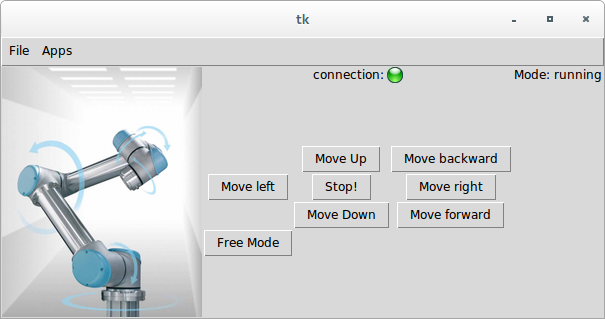
\includegraphics[width=0.8\textwidth]{pic/hda_urcontrol_gui.png}
      \caption[Selbsterstelltes GUI zur Steuerung des UR5 Roboters]{Startfenster des selbst erstellten GUIs zur Steuerung des UR5 Roboters. Der Roboter lässt sich in alle Richtungen linear bewegen.}
      \label{fig:hda_urcontrol_gui}
\end{figure}

\subsection{Test und Fehlersuche im Programm}
\label{debuggen_mit_hoeherer schicht}

Nach Ausschluss der Fehler im Adapter, ist es möglich Unittests\footnote{Unittests erlauben es einzelne Komponenten/Module in einem Programm zu Testen} für das Programm zu benutzen. Die Schnittstelle zum Roboter wird hier durch einen sogenannten Mock\footnote{Ein Platzhalter für Software-Objekte. Wird benutzt, um Software zu testen, bei der ein Teil der Software noch nicht existiert oder ausgeschlossen werden soll.} erstetzt. Dadurch kann auch offline getestet werden. Fehler werden in den etablierten Programmiersprachen so einfach gefunden und lokalisiert. In etablierten Programmiersprachen, sei es eine Sprache die mit einem Interpreter arbeitet oder vorher kompiliert wird, wird vor der Ausführung die Syntax getestet. Deshalb können auch Syntaxfehler im Gegensatz zur URScript-Sprache lokalisiert werden.

\subsection{Aufwand der Programmierung}
\label{eigene_api_aufwand}

Der Aufwand für ein Programm ist mit einer eigenen API anfangs deutlich höher gegenüber den anderen Methoden. Es muss erst ein Adapter geschrieben und getestet werden, bevor die eigentliche Anwendung geschrieben werden kann. 
Nach dieser Hürde, lassen sich jedoch unkompliziert Programme erstellen, die auf den Adapter zugreifen, um den Roboter zu steuern.
 \chapter{Ergebnis}
\label{sec:ErreichteErgebnisse}

Im Folgenden Kapitel werden die Schnittstellen werden gegenübergestellt und verglichen. Desweiterem werden die nicht erreichten Ziele erörtert.
\\\\
\begin{tabular}{|l|p{0.333\textwidth}|p{0.333\textwidth}|}
	\hline
	\textbf{Kriterium} & \textbf{C-API} & \textbf{Polyscope} 
	\\ \hline \hline 
	Programmierbarkeit & Schwer einfache Roboterprogramme zu Realisieren. & Leichter Einstieg zum Programmieren für Anfänger.
	\\ \hline
	Benutzerinteraktion &  Es ist möglich ein Übersichtliches \& intuitives Interface zu entwickeln & 
	Keine Komplexen Menüs möglich. Nur schwache Interaktion möglich.
	\\ \hline
	Testen & Test sind möglich, aber nur mit Simulation des Roboters & Keine eigenen Tests möglich. Getestet wird immer Live an Roboter.
	\\ \hline
	Debuggen & Compiler findet Syntax Fehler \& Debugging ist nur mit Simuliertem Roboter möglich & Bedingt möglich beim Testen Live am Roboter.
	\\ \hline
	Aufwand & Sehr großer Aufwand von nöten. Es muss alles selbst Entwickelt werden. & \label{krit_polyscope_aufwand}
	Bei kleinen Programmen kaum Aufwand. Aufwand steigt enorm bei mehr Anforderungen.\\ \hline
\end{tabular}
\captionof{table}{Zusammenfassung der Evaluierungskriterien für C-API und Polyscope}
\label{tab:vgl_interfaces_first}

\begin{tabular}{|l|p{0.33\textwidth}|p{0.33\textwidth}|}
	\hline
	\textbf{Kriterium} & \textbf{URScript} & \textbf{Eigener Adapter}\\ \hline \hline 
	Programmierung & verständnissvolle Dokumentation ermöglicht es einen schnellen Einstieg. Entwicklerwerkzeuge und \ac{Syntax Highlighting} erleichtern die Übersicht und Vereinfachen die Programmierung & Eine Etablierte Programmiersprache erleichtert das Programmieren deutlich. Vorhandene \acl{Librarys} erleichtern das Programmieren. \\
	\hline 
	Benutzerinteraktion & Die möglichkeiten bleiben wie bei Polyscope mit Popups beschränkt(siehe \ref{user_interaktion_polyscope_rel}) & Wie bei C-\ac{API} können \ac{GUI}'s erstellt werden, die komplexe Formulare und Menüs bieten. \\
	\hline 
	Testen & Mit gegebenen Mitteln sind automatische Tests nicht möglich. Es kann nur wie mit Polyscope Live getestet werden. & Automatische Test sind möglich. \\
	\hline
	Debuggen & Es gibt keine Möglichkeit zu Debuggen. URController liefert bei Fehler in der Syntax keine information & Fehler werden leicht gefunden, da die Etablierten Programmiersprachen den Programmcode nach Syntaxfehlern durchsuchen und anzeigen.
	\\
	\hline 
	Aufwand & Ähnlich wie bei Polyscope, jedoch etwas besser durch mehr Übersicht des Projektes & Anfangs ein Großer Aufwand von nöten. Bei mehreren Anwendungen für den Roboter ist Aufwand jedoch geringer als bei den anderen Schnittstellen.\\ 
	\hline 
\end{tabular}
\captionof{table}{Zusammenfassung der Evaluierungskriterien für URScript und Eigener Adapter}
\label{tab:vgl_interfaces_second}

\section{Vergleich der Schnittstellen}

Die C-API ist eine sehr Hardware nahe Schnittstelle zum Roboter. Der Aufwand der Betrieben werden muss ist sehr hoch. Diese Schnittstelle sollte nur in seltenen Fällen eingesetzt werden. Nur Spezielle Anwendungen die zur Laufzeit anpassungen an Bewegungssteuerung geben sollten diese Schnittstelle nutzen.
\\\\
Die Polyscope Software ist sehr gut geeignet für wenige komplexe Anwendungen, die keine bzw. kaum Benutzerinteraktion erfordern. Für eine Kollaboration die auf Interaktion angewiesen ist, ist diese Schnittstelle nicht zu empfehlen. Diese Schnittstelle kann nur sehr aufwändig auf persistente Daten zugreifen und speichern.
\\\\
URScript bietet in sachen Benutzerinteraktion nur die gleichen möglichkeiten, wie die Polyscope Software(siehe \ref{ur_script_user_interaction}). Es ist Übersichtlicher und verständlicher gegenüber Polyscope Anwendungen zu entwickeln, jedoch bietet die eigens entwickelte Scriptsprache nur wenig möglichkeiten, wirklich komplexe Anwendungen zu entwickeln.
\\\\
Der Eigene Adapter zum URController vereint die Vorteile einer etablierten Programmiersprache, nämlich vorhandene Entwicklerwerkzeuge und \ac{Software Bibliotheken} zu nutzen. Der Roboter wird über URScriptbefehle gesteuert wird, deshalb muss nicht tief in die Robotersteuerung eingreifen werden wie bei der C-API. Wenn viel Benutzerinteraktion von nöten ist, ist diese Schnittstelle zu empfehlen.

\section{Nicht erreichte Ziele}
\label{sec:Nicht_erreichte_ziele}

Mit der C-API konnte keine Anwendung geschrieben werden, die für die Evaluierungskriterien vollständige Daten liefern.
 \chapter{Fazit}

\section{Zusammenfassung}
\label{sec:Zusammenfassung}

Der Beste weg für die Kollaboration ist einen eigenen Adapter in einer Programmiersprache zu schreiben um Programme mit richtigen \ac{GUI}'s zu entwickeln.
\\\\
\textbf{Polyscope}\\
Die Polyscope Schnittstelle bietet keine Möglichkeiten, diese zu erweitern. Die möglichkeiten für die Kollaboration sind hier auch sehr gering. Diese Schnittstelle kann nur benutzt werden um kleine und wenig Komplexe Programme zu schreiben.
\\\\
Die URScript Sprache ist ein wenig angenehmer zu Programmieren als die Polyscope Software, jedoch bleiben die möglichkeiten der Kollaboration genauso beschränkt.
\\\\
Die C-\ac{API} bietet nur wenig Möglichkeiten zur Steuerung des Roboters. Wenn die hürden überwunden sind, ist es jedoch möglich wie mit dem eigenen Adapter über \ac{GUI}'s mit dem Roboter zu Kollaborieren.

\section{Ausblick}
\label{sec:ausblick}

\textbf{URScript}\\
Das Programm, dass für die Beispielanwendung geschrieben wurde um URscript Programm an den Roboter zu senden, kann erweitert werden. Es ist möglich den Pre-Processor so zu erweitern, dass die URScript Sprache mit Funktionen erweitert wird, in dem Textstellen ersetzt werden. Zusätzlich kann man die Syntax überprüfen, um Fehler in der Syntax früh zu erkennen.
\\\\
\textbf{Eigener Adapter}\\
Der Adapter kann un unzähliche möglichkeiten erweitert werden. Komplexe Strukturen in der URScriptsprache können leicht abstrahiert werden und mit dem Adapter umgesetzt werden. Es ist möglich auch andere Programmiersprachen zu nutzen. Als Vorbild könnte der geschriebene Adapter dienen. Am Besten geeignet, sind aber schnelle Programmiersprachen. Der Roboter sendet im 60hz Takt die Daten an den Adapter, da wäre es nicht sinnvoll, wenn das \ac{parsen} der Daten zu lange dauert.
\\\\
\textbf{C-API}\\
Mit der Beispielanwendung ist ein kleiner Schritt getan, um über die C-API den Roboter zu steuern, jedoch müssen erst die aufgetretenen Fehler behoben werden.
 
 \clearpage
 \appendix
 
 \begin{thebibliography}{XXXXXX-JJJJa}

\bibliography{Literatur/quellen}

\renewcommand{\bibname}{A. ~Literaturverzeichnis}
\addcontentsline{toc}{chapter}{\protect\numberline{A}{Literaturverzeichnis}}
\setcounter{chapter}{1}

%\addcontentsline{toc}{chapter}{A. ~Literaturverzeichnis}

%\bibitem [DJAN-2013]: Organisation/Hersteller/Autor: Titel [: Untertitel].
%\url{URL}, [Datum, sofern auf Web-Seite angegeben], zuletzt besucht am Datum.
%(Internet)

\bibitem [WW-2013]{WW-2013} Weber, Wolfgang: Industrieroboter: Methoden der Steuerung und Regelung. 2.Auflage, Carl Hanser Verlag GmbH \& Co. KG, München, 2007.
\bibitem [ROSPR-2013]{ROSPR-2013} ROS.org/PascalRey: ROS Wiki: Documentation. \url{http://wiki.ros.org/}, 2013-12-17 14:34:30, zuletzt besucht am 25.03.2014
\bibitem [DINISO-2012]{DINISO-2012} DIN EN ISO 10218-1:2012-01 : Industrieroboter: Sicherheitsanforderungen - Teil 1 Deutsche Fassung \url{http://www.beuth.de/de/norm/din-en-iso-10218-1/136373717}, 2012-01, zuletzt besucht am 25.03.2014
\bibitem [MATLAB-2014]{MATLAB-2014} Mathworks.de: Matlab: Die Sprache für technische Berechnungen \url{http://www.mathworks.de/products/matlab/}, zuletzt besucht am 27.03.2014
\bibitem [TK-2014]{TK-2014} PaulBoddie: Python Tkinter: Introduction. \url{https://wiki.python.org/moin/TkInter}, 2014-01-16 19:41:50, zuletzt besucht am 25.03.2014
\bibitem [CP-2014]{CP-2014} falvarezcp2008: C Programming: How to set a socket connection timeout. \url{http://www.codeproject.com/Tips/168704/How-to-set-a-socket-connection-timeout},  03.2011, zuletzt besucht am 25.03.2014
\bibitem [GMM-2014]{GMM-2014} Gordon McMillan: Python: Socket Programming HOWTO. \url{http://docs.python.org/2/howto/sockets.html}, zuletzt besucht am 25.03.2014
\bibitem [DOCP-2014]{DOCP-2014} docs.python: Python Struct: Interpret strings as packed binary data. \url{http://docs.python.org/2/library/struct.html}, zuletzt besucht am 25.03.2014

%\bibitem [DJAN-2013]: Name1, Vorname1[; Name2, Vorname2; ...]: Titel [: Untertitel]. In: Tagungsband, Herausgeber, Bezeichnung der Tagung, ggf. Ort und Fachgesellschaft, S. xx - yy. (Tagungsbänden)
%\bibitem [DJAN-2013]: Name1, Vorname1[; Name2, Vorname2; ...]: Titel [: Untertitel]. In: Zeitschriftentitel Jahrgangnummer(Jahreszahl)Heftnummer, S. xx - yy.  (Zeitschriften)
%\bibitem [DJAN-2013]: Organisation/Hersteller/Autor: Titel [: Untertitel]. \url{
% (Internet)

\end{thebibliography}% 
  \chapter{Glossar}
 \label{sec:Glossar_glo}

\begin{acronym}[Syntax Highligting]%% in [] längste zu erwartende Abkürzung
%\setlength{\itemsep}{-\parsep}
 
 \acro{Syntax Highligting}{} Zur Verbesserung der Lesbarkeit und der Übersicht, wird in einem Textverarbeitungsprogramm der Programmcode unterschiedlich dargestellt. Meist mit unterschiedlichen Farbwerten. Der Entwickler sieht mit einem Blick ob er es mit Textvariablen, Zahlenwerten zu tun hat.
 \acro{ISO}{International Organization for Standardization}: Die ISO ist eine Internationale Vereinigung um Standartisierte Normen in der Industrie zu erarbeiten und festzulegen. Jedes Land, dass Mitglied ist, muss sich an diese Normen halten. Es gibt fast kein Land, dass nicht Mitglied ist.
 \acro{PTP}{Point to Point}: PTP in Deutsch auch Punktsteuerung genannt, ist die einfachste Methode um einen Roboter auf einen anderen Zielpunkt zu fahren.
 \acro{API}{Application Programming Interface}: Eine Schnittstelle um eine Software mit einer anderen Software zu verbinden. Die Schnittstelle in Form eines Programmteils wird öffentlich gemacht und gut Dokumentiert. Die Externe Software benutzt diesen Programmteil um die Software mit der Schnittstelle zu nutzen.
 \acro{URP}{Univeral Robot Program}: URP ist eine Dateiendung für ein Programm geschrieben über die Polyscope Software.
 \acro{UR}{Universal Robots}: UR ist eine Dänische Firma die den UR5 Roboter Herstellt.
 \acro{Library}{Software Bibliotheken}: Eine Software Bibliothel, oft auch Modul oder Library genannt, ist eine Kapselung von Programmcode der wiederverwendet werden kann.
 \acro{TCP/IP}{Transmission Control Protocol / Internet Protocol}: TCP/IP ist beinhalten mehrere Netzwerkprotokolle, die es ermöglichen, dass man mehrere Rechner Vernetzen und Nachrichten austauschen lassen.
 \acro{Popup}{} Ein Fenster oder anderes Visuelles Element um einem Benutzer einer Anwendung Nachrichten zukommen zu lassen.
 \acro{parsen}{Parser}: Parser: Informationen zerlegen und entsprechend interpretieren.
 \acro{Mock}{} Ein Platzhalter für Software Objekte. Wird benutzt um Software zu testen, bei dem ein Teil der Software noch nicht existiert oder ausgeschlossen werden soll.
 \acro{Interpreter}{} In der Softwareentwicklung sind Interpreter die Kernpunkte von Programmiersprachen die den Code nicht in Machinensprache Kompilieren. Interpreter lesen den Textcode analysieren ihn auf fehler und führen ihn nach der Analyse aus.
 \acro{Big-Endian}{Big-Endian Format}: Big Engian Format ist die Festlegung der Byte-Reihenfolge, wie das Computersystem Speicherbereiche interpretieren und beschreiben soll. Dieses Format legt fest, dass das höchstwertigste Bit an der kleinsten Speicheradresse liegt.
 \acro{Little-Endian}{Little-Endian Format}: Wie bei \acs{Big-Endian Format}, legt das Little-Endian Format die Byte-Reihenfolge fest. Mit Little-Endian jedoch wird das niedrigwertenste Bit an die kleinste Speicheraddresse gesetzt.
 \acro{ROS}{Robot Operating System}: ``Provides libraries and tools to help software developers create robot applications. It provides hardware abstraction, device drivers, libraries, visualizers, message-passing, package management, and more. ROS is licensed under an open source, BSD license.'' \cite{ROSPR-2013}
 \acro{Queue}{} Eine Warteschlange, ähnlich wie bei einem Supermarkt. Die Elemente in einer Queue werden Nacheinander abgearbeitet. 
 \acro{TCP}{Tool Center Point}: Der TCP beschreibt den Punkt des Werkstücks, der auf den Roboter Montiert ist. In der Regel ist dieser Punkt an der Spitze des Werkzeugs angeben.
 \acro{teachen}{}: In der Robotik ist teachen, das Anlernen von Wegpunkten, durch handliches führen am Roboter.
 \acro{SCP}{Secure Copy}: Ein Linux Programm zum Sicheren austauschen von Daten zwischen zwei verschiedenen Host-Systemen
 \acro{GUI}{Graphical User Interface}: Ein GUI erlaubt es einen Benutzer mit einem Programm über graphische Symbole zu Interagieren
 \acro{Unittest}{}: Unittests erlauben es einzelne Komponenten/Module in einem Programm zu Testen
 \acro{Socket}{}: Ein Socket ermöglichen ein Datenaustausch zwischen Programmen im Rechner oder auch zwischen 2 verschiedenen Host Systemen
 \acro{USB}{Univeral Serial Bus}: Mit USB kann man den Rechner mit externen Systemen verbinden und Daten austauschen.
 % \acro{}{}:
\end{acronym}

 \chapter{Quellcode}
\label{quellcode}

\section{Bewegungsprofile geloggt über die Echtzeitschnittstelle \& geplottet in Matlab}
\label{sec:profile_polyscope_rci}

\begin{figure}[H]
  \centering
    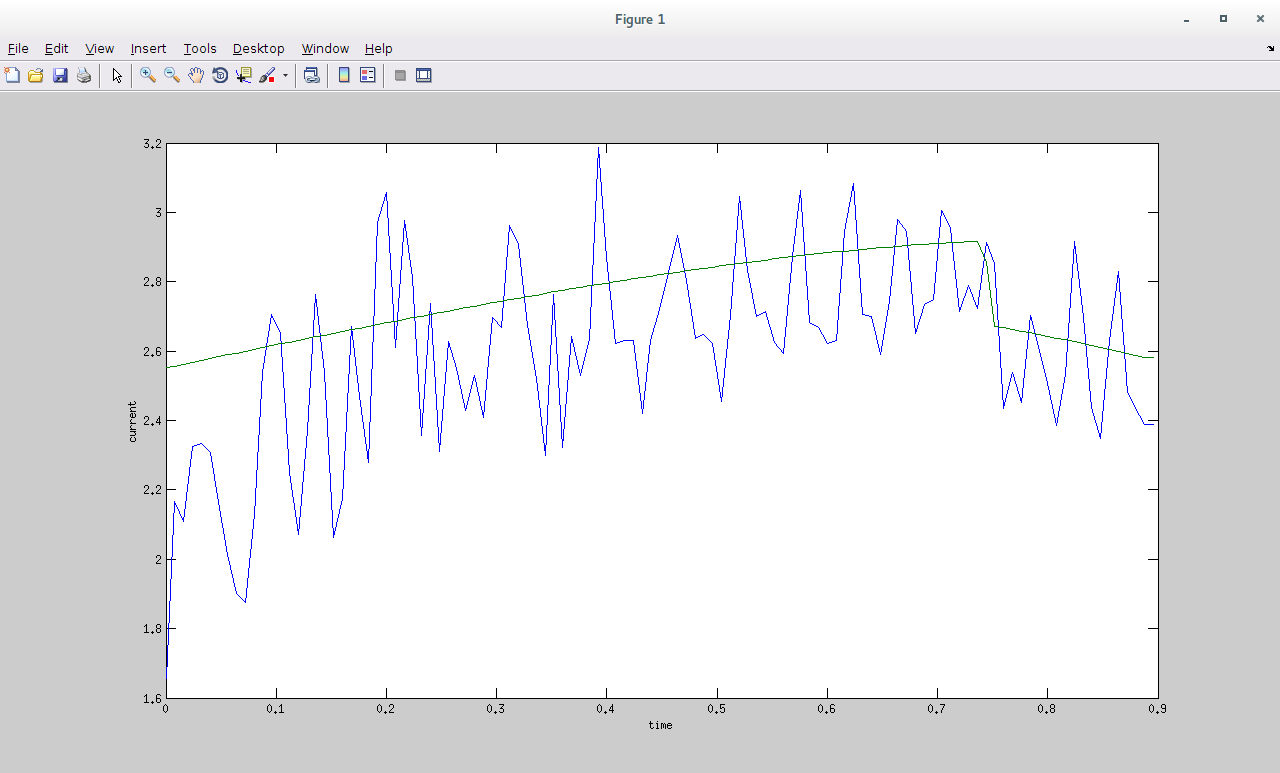
\includegraphics[width=0.8\textwidth]{pic/joint3_current_polyscope.png}
      \caption[Stromstärke wärend der Bewegung des 3. Gelenks]{}
      \label{fig:acceleration_profile_rci}
\end{figure}

\begin{figure}[H]
  \centering
    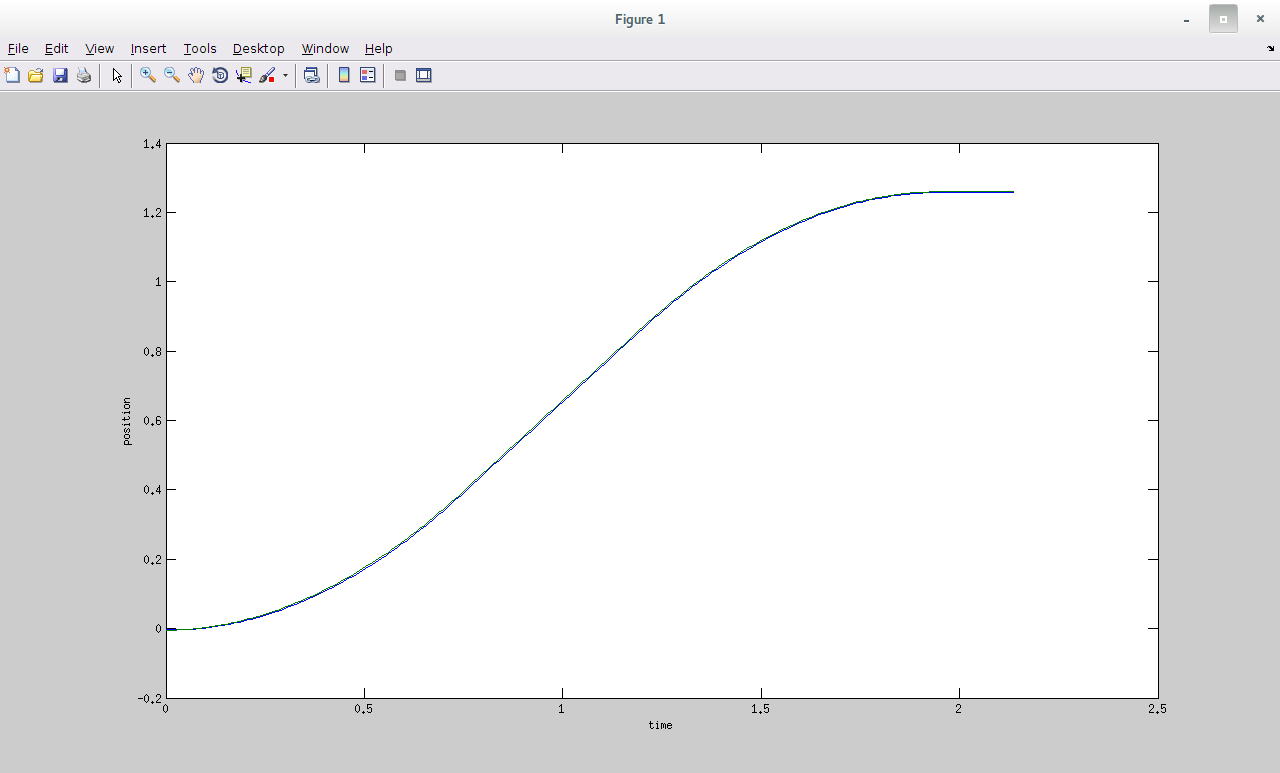
\includegraphics[width=0.8\textwidth]{pic/joint5_position_polyscope.png}
      \caption[Position der Soll und Ist Werte für das 5. Gelenk]{}
      \label{fig:position_joint5_rci}
\end{figure}

\section{Bewegungsprofile geloggt in der C-\ac{API}}
\label{sec:profiles_with_capi}

\begin{figure}[H]
  \centering
    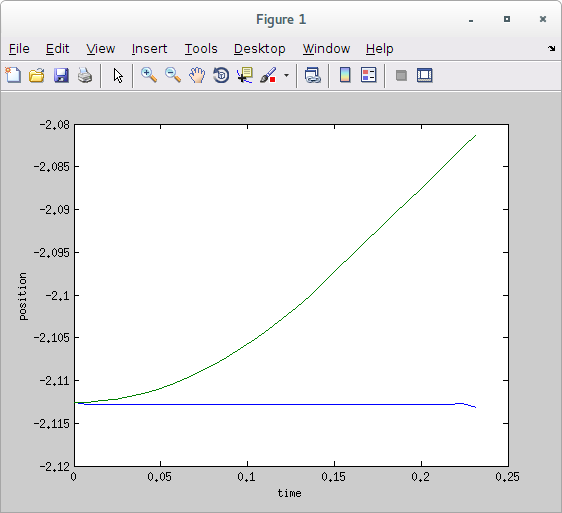
\includegraphics[width=1\textwidth]{pic/joint1_position_capi.png}
      \caption[Soll und Ist Werte der Position des 2.Gelenks]{}
      \label{fig:joint_1_position_capi}
\end{figure}

\begin{figure}[H]
  \centering
    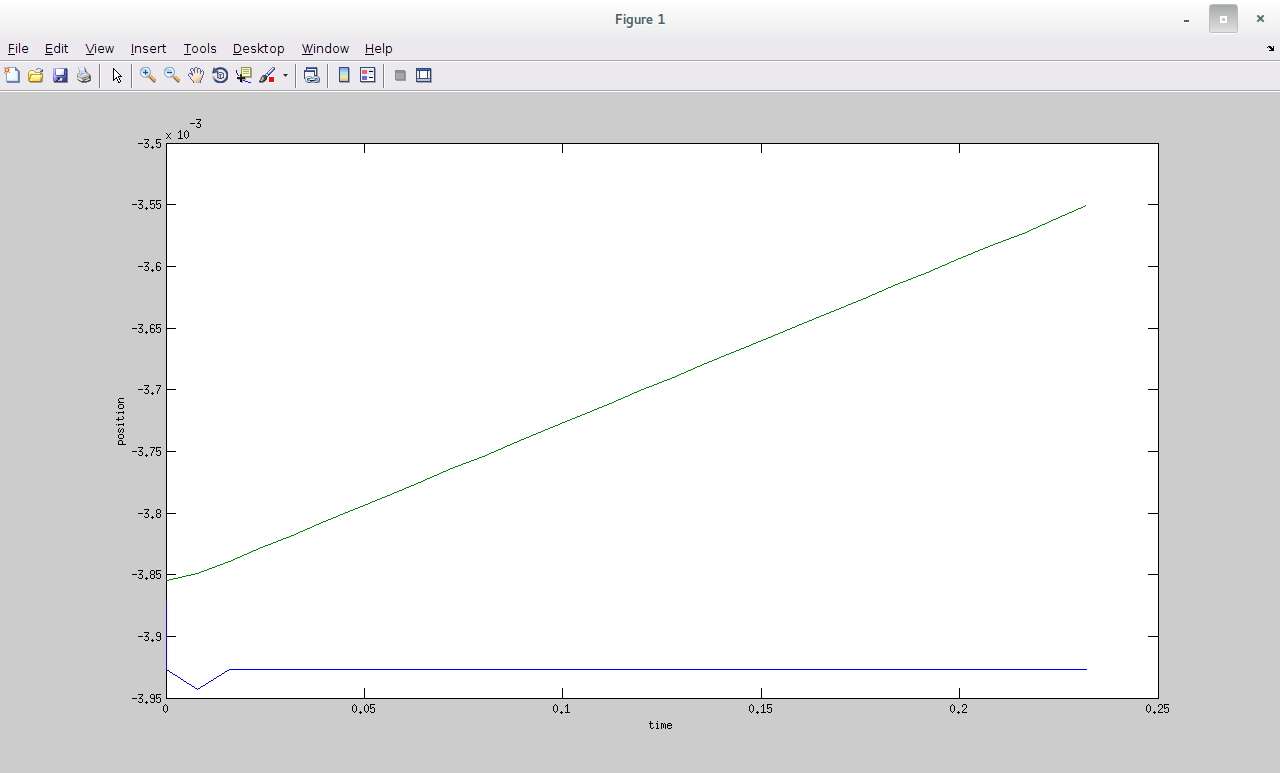
\includegraphics[width=1\textwidth]{pic/joint5_position_capi.png}
      \caption[Position der Soll und Ist Werte für das 5. Gelenk]{}
      \label{fig:position_joint5_capi}
\end{figure}

\section{Speichern der Daten über TCP in der Datenbank}
\label{save_data_tcp_code_gru}

\begin{lstlisting}
#!/usr/bin/env python2.7

from my_utils import connection, Player, get_ip
import socket
import signal
import sys
import os

class SaveDataInterface():
    def __init__(self, interface="localhost"):
        self.__run_flag=False
        self.interface = interface
        self.socket=socket.socket(socket.AF_INET, socket.SOCK_STREAM)
        ip = get_ip(interface)
        if ip is None:
            ip="127.0.0.1"
        else:
            ip = get_ip(interface)
        port = 8000
        self.socket.setsockopt(socket.SOL_SOCKET, socket.SO_REUSEADDR, 1)
        try:
            self.socket.bind((ip, port))
            print "server is listen on %s:%d" %(ip, port)
            self.socket.listen(1)
        except socket.error, e:
            print(e[0])
            self.socket.close()
            self.socket=None

    def run(self):
        self.__run_flag=True
        # print("starting send interface waiting for queue")
        while self.__run_flag:
            if self.socket is not None:
                conn, addr = self.socket.accept()
                conn.settimeout(2)
                print "client connected: {0}".format(addr)
                player=None
                while self.__run_flag:
                    msg = self.read_from_socket(conn)
                    if msg is not None:
                        if msg == "new_patient":
                            # print("wait for new patient name")
                            name = self.read_from_socket(conn)
                            player = connection.Player()
                            player.name = name.rstrip()
                            player.save()
                        elif msg == "load_patient":
                            print("wait for patient name")
                            name = self.read_from_socket(conn)
                            player = connection.Player.find_one({'name': name.rstrip()})
                            if player is not None:
                                print("send %s"%"1".encode('ascii'))
                                print("positions %s"%("(%s)"%player.start_pos[1:-1]).encode('ascii'))
                                conn.send("(1)".encode('ascii'))
                                conn.send(("(%s)"%player.start_pos[1:-1]).encode('ascii'))
                            else:
                                conn.send("(0)".encode('ascii'))
                        elif msg == "set_patient_data":
                            # print("wait for player data")
                            start_position = self.read_from_socket(conn)
                            player.start_pos=start_position.rstrip()
                        else:
                            print("recieved unknown command")
                    else:   
                        break
                conn.close()

        self.socket.close()
        return 0

    # This Function reads from the Socket conn the next msg checks for errors
    def read_from_socket(self, conn):
        msg = None
        while self.__run_flag:
            try:
                msg = conn.recv(1024)
            except socket.timeout, e:
                err = e.args[0]
                # this next if/else is a bit redundant, but illustrates how the
                # timeout exception is setup
                if err == 'timed out':
                    # print 'recv timed out, retry later'
                    continue
                else:
                    print e
                    msg=None
            except socket.error, e:
                print e
                msg=None
            else:
                if len(msg) == 0:
                    msg=None
                    break
                else:
                    print msg
                    break
        return msg


sdi = SaveDataInterface(interface="eth0")

sdi.run()
\end{lstlisting}

 
\end{document}